
\noindent {\bf Objectives}:
\begin{itemize}
\item To understand the concept of \emph{color} in astronomy.
\item  To be able to classify galaxies based on their morphology and colors
\item  To investigate how galaxies evolve over time
\item  To search for, analyse and interpret information from large galaxy surveys including the Sloan Digital Sky Survey (SDSS)
\end{itemize}

\noindent
%{\bf Part 1. Virgo Cluster}
{\bf  Introduction}:

\begin{figure*}[ht]
        \begin{center}{\psfig{figure={Hubblefork.eps},width=10.0cm}}
        \caption{Hubble’s famous Tuning Fork diagram created by Dr Karen Masters, based on an activity designed by Las Cumbres Observatory Global Telescope Network (LCOGT).}\label{hubblefork}
        \end{center}
                \end{figure*}

\noindent

Edwin Hubble created the first classification of galaxies. He produced
a diagram, called the Tuning Fork diagram (Figure \ref{hubblefork})
based on features galaxies have in common. He came up with three
distinct groups - ellipticals, spirals and irregulars. Ellipticals
have no spiral arms or a disk and are classified by how round they
look, E0 is very round but an E7 is very flat. This number is actually
the ellipticity of the galaxy (the ratio of the semi major axis to the
semi minor axis). Spirals show a spiraling structure, spiral ``arms'',
and can be further split into barred (SB) and un-barred (S). They are
also classified by how tight their spiral arms are ``wound''. There is
a transition type called S0 which have no spiral arms but they have a
central bulge and a disk. Astronomers now use a slightly different
naming system with two major groups called early-type (including
ellipticals and S0s) and late-type galaxies (spirals).

Hubble thought that galaxies in time moved from left to right in his
Hubble Tuning Fork diagram over time, but we now know that this is
incorrect. Some galaxies move from right to left over time, and a much
smaller number from left to right sometimes, but there is no
inevitable progression of any individual galaxy across the diagram.

\noindent{\bf 2. The color of galaxies}

\noindent

The Sloan Digital Sky Survey SDSS has imaged a large portion of the
sky, and found more than 80 million galaxies. Classifying them by eye
would take huge amount of time. SDSS cleverly called upon the public
to help, and asked volunteers to look at images of new galaxies,
compare them with typical Early and Late type galaxies, and classify
the new objects accordingly. This project is called the \emph{Galaxy
Zoo}, {\tt http://www.galaxyzoo.org}. A quicker way to classify
galaxies, easier to implement in a computer, is by using their color.

\noindent {\bf Question:} Look at the Hubble Tuning Fork diagram reproduced above. How does the color differ for different galaxy types?



\begin{figure*}[ht]
        \centerline{\psfig{figure={SDSSgals.eps},width=18.0cm}}
        \caption{A selection of SDSS galaxies. }\label{SDSSgals}
         \end{figure*}


\noindent 
Figure \ref{SDSSgals} shows a selection of SDSS galaxies. The SDSS survey takes sky images in multiple filters. By combining these images color images of astronomical objects are obtained. 

\noindent First, look at each galaxy in Figure \ref{SDSSgals} and classify it according to its \emph{shape} according to both classification schemes: as \emph{early} or \emph{late} type, and as \emph{elliptical} E0-6, S0, \emph{spiral} S or SB a,b or c.

\vspace{20pt}

\noindent a \makebox[2cm]{\hrulefill}  \makebox[2cm]{\hrulefill}\makebox[1cm] d \makebox[2cm]{\hrulefill}  \makebox[2cm]{\hrulefill}\makebox[1cm] g \makebox[2cm]{\hrulefill}  \makebox[2cm]{\hrulefill}

\noindent b \makebox[2cm]{\hrulefill}  \makebox[2cm]{\hrulefill}\makebox[1cm] e \makebox[2cm]{\hrulefill}  \makebox[2cm]{\hrulefill}\makebox[1cm] h \makebox[2cm]{\hrulefill}  \makebox[2cm]{\hrulefill}

\noindent c \makebox[2cm]{\hrulefill} \makebox[2cm]{\hrulefill}\makebox[1cm] f \makebox[2cm]{\hrulefill}  \makebox[2cm]{\hrulefill}\makebox[1cm] i \makebox[2cm]{\hrulefill}  \makebox[2cm]{\hrulefill}

\vspace{20pt}


\noindent Now go to the SDSS Object Explorer Tool:

\noindent {\tt http://cas.sdss.org/public/en/tools/explore/obj.aspx}

\noindent and type in their coordinates (``Search by,'' at top
left). Click ``Save to Notes'' for each galaxy to save the information
automatically. Then you can just click on ``Show Notes'' to see your
measurements.  I mentioned that SDSS observed in \emph{multiple
filters} to obtain color information about astronomical objects. The
SDSS filters are: \u, \g, \r, \i \ and \z; \u \ is the bluest filter
and \z \ is the reddest.

\noindent 
You want to make a \emph{color-color diagram} of these galaxies. A
color-color diagram is a very useful astronomical tool: it is a plot
of one particular color, against another, for the same object.  In
astronomy colors are defined as difference in magnitude in different
filters. For this particular color-color diagram you want to plot the
SDSS \g-\r \ color, against the \u-\g \ color, i.e. \u-\g \ is on your
$x$-axis, \g-\r \ is on the $y$-axis. Now pay attention: because you
are using magnitudes, where the larger the number the brighter the
object, this may be counterintuitive:

\noindent {\bf Question:} Which is bluer: a galaxy with a larger value of \u-\g \ or with a lower value of \u-\g?

\noindent 
Use the box below for your color-color diagram. Mark the bottom-left
and top-right corner with the word BLUE or RED according to where you
expect the bluest and the reddest objects to fall. Draw an arrow that
indicates the direction in the plot in which objects get redder.

\noindent
Plot your \g-\r \ vs \u-\g \ colors in the box below. Briefly note
whether you see any patterns.


\begin{figure}[b!]
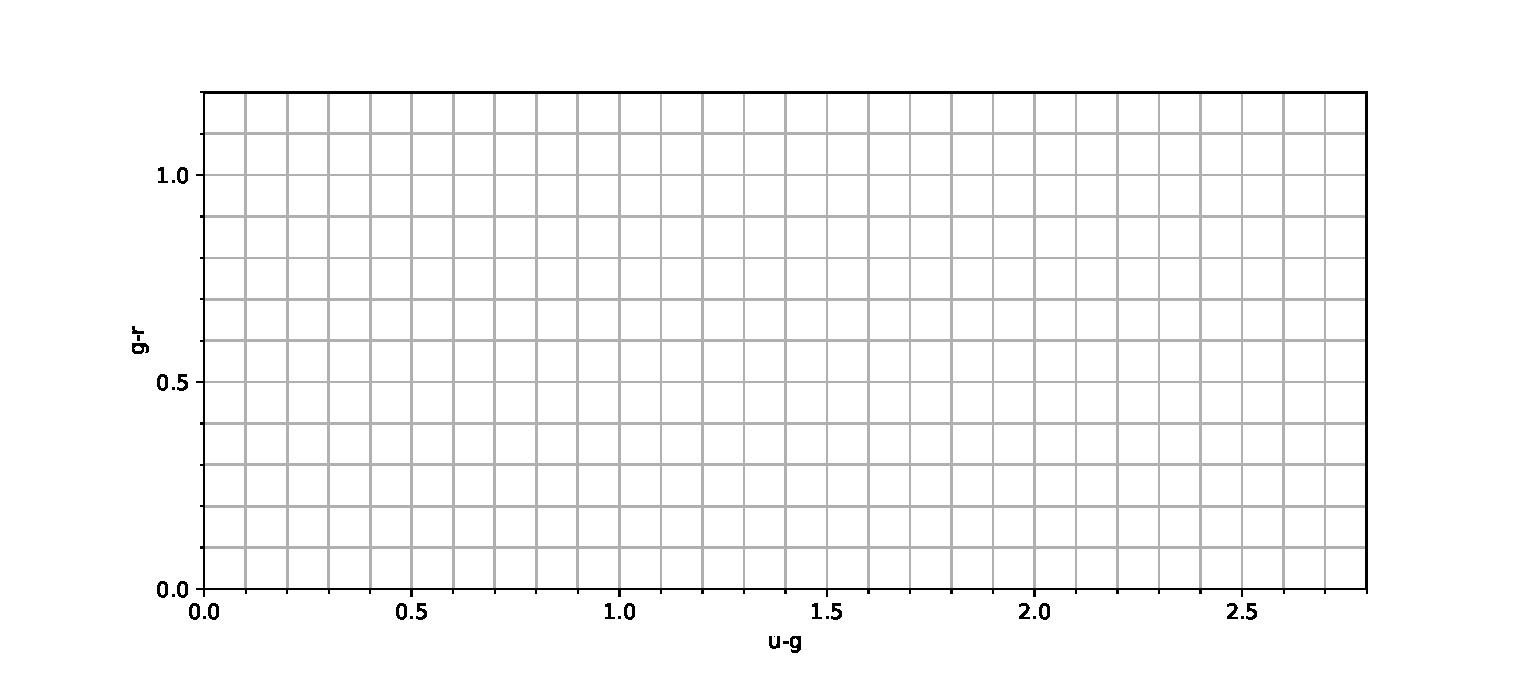
\includegraphics[width=0.99\textwidth]{colorcolor.eps}
\end{figure}

\clearpage

\noindent
Now draw a line $$y=-x+2.2.$$ This means draw a line the join points
that have $y$-axis value equal to 2.2 - the $x$-axis value. It was
found studying the SDSS sample that early type galaxies have ($u-r$)
values higher than 2.2, and late type galaxies have ($u-r$) values
lower than 2.2, indeed they are split by the equation ($g-r$) = $- (u-g)
+ 2.2$ (Strateva et al. 2001). Do you see this pattern in the data you analyzed? 

\bigskip
\noindent
Mark the box regions according to the type you expect them to host in the plot: mark the regions above and below your $y=x+2.2$ line with either EARLY or LATE, whichever you think is appropriate. 

%\begin{center}{\bf Extra credits/Homework}\end{center}

\noindent
{\bf 3. Clusters of galaxies}:

\noindent
George Abell classified \emph{thousands} of galaxy clusters, publishing them in 1958. We will use a few of them to see how galaxy colors change with redshift and draw conclusions about galaxy evolution!
The galaxy cluster Abell 2255 is at co-ordinates RA = 258.1292\deg\  and Dec = 64.092\deg .

\noindent
To obtain the colors of galaxies in Abell 2255, use the SDSS archive Navigation Tool: 

\noindent{\tt http://cas.sdss.org/public/en/tools/chart/navi.aspx}.

\noindent
You will need to type in the coordinates of the Abell 2255, click on ``Get Image'' and zoom out once or twice. Now click on roughly 20 galaxies that you think are part of the cluster (make a note of what criteria you use to decide if these are cluster members). On the right hand side of this webpage, you will see the colors listed for the galaxy you clicked on, write these down. You can click Save to Notes for each galaxy to do this automatically or do it by hand by typing/writing them. If you save the notes on the webpage just click on ‘Show Notes’ to see your measurements. You can export to CSV format if you wish to work on it in Excel, or any computational language, but that is not necessary.
Don’t forget, however, to include all of your measurements in your lab diary (stapled print-outs are fine).

\noindent
Important: think carefully about how you know which galaxies are part of Abell 2255, and which are just other galaxies at different distances in the same part of the sky. Briefly describe your 20 galaxies. Are they similar? How are they different? Make a color-color plot (as above) of your sample of Abell 2255 galaxies. Again, draw the line that ‘separates’ ellipticals from spirals. How many of these galaxies are ellipticals and how many spirals?



\clearpage

%\noindent
%{\bf Do Galaxy Colors Change with Redshift?}
%
%\noindent
%Now you have done this for a relatively nearby cluster (at a redshift of 0.081), try comparing the colors and classification of galaxies in clusters at different redshifts. The table below provides coordinates and redshift information fot three Abel clusters:
%
%\begin{table}[ht!]
%\begin{center}
%\begin{tabular}{l c c c}
%Name of cluster &  Redshift & RA (deg) & Dec (deg)\\\hline
%Abell 2255 & 0.081 & 258.129 & 64.093 \\ 
%Abell 0023 & 0.105 & 5.44 & -0.89 \\
%Abell 0267 & 0.230 & 28.77 & 1.01
%\end{tabular}
%\end{center}
%\caption{ Properties of the galaxy clusters used in this research project.}
%\end{table}
%
%\noindent
%Follow the same procedure as before to get the SDSS data on each cluster and create color-color plots. You will have to assume your sample contains no foreground or background galaxies. Count the \emph{fraction} of Early and Late type galaxies in each cluster. 
%\begin{itemize}
%\item{How does it change with the redshift? }
%\vspace{30pt}
%\item{What does that mean?}
%\vspace{30pt}
%\item{Can you comment in the light of this result on Hubble's initial prediction, that Galaxies would evolve rightward in his plot?}
%\vspace{30pt}
%\item{ Can you relate this result to what you know about \emph{stellar} evolution?}
%\end{itemize}

